\begingroup
\renewcommand{\baselinestretch}{1}\selectfont
% Local, reusable vector figure styles. Units are centimetres.
\tikzset{
 thesis block/.style={draw=black,line width=.65pt,align=center,inner sep=5pt,font=\sffamily\fontsize{10}{12}\selectfont},
 thesis hw/.style={thesis block,fill=black!9},
 thesis sw/.style={thesis block,fill=white},
 thesis memory/.style={thesis block,double,double distance=1pt,fill=black!3},
 thesis arrow/.style={->,>=stealth,line width=.7pt},
 thesis transfer/.style={<->,>=stealth,line width=.7pt},
 thesis note/.style={align=center,font=\sffamily\fontsize{9}{11}\selectfont,inner sep=3pt},
 thesis title/.style={thesis note,font=\sffamily\bfseries\fontsize{10}{12}\selectfont}
}

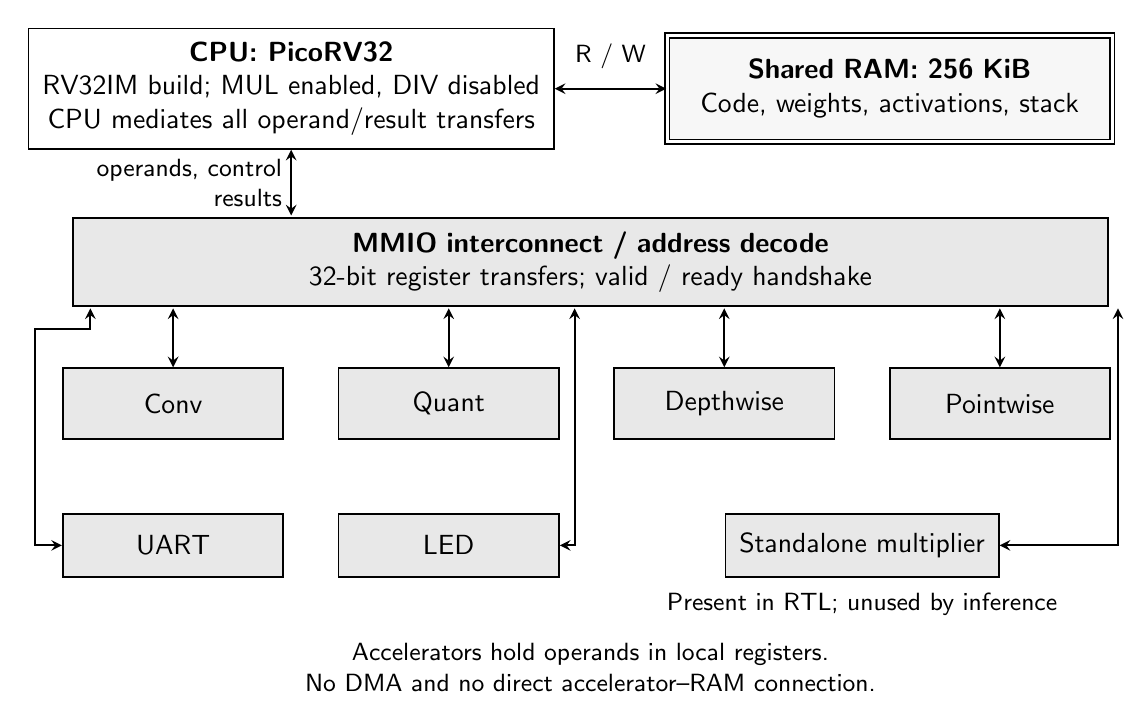
\begin{tikzpicture}[x=1cm,y=1cm]

\node[thesis sw,minimum width=5.2cm,minimum height=1.35cm] (cpu) at (3,0) {\textbf{CPU: PicoRV32}\\RV32IM build; MUL enabled, DIV disabled\\CPU mediates all operand/result transfers};
\node[thesis memory,text width=5.3cm,minimum height=1.35cm] (ram) at (10.6,0) {\textbf{Shared RAM: 256 KiB}\\Code, weights, activations, stack};
\draw[thesis transfer] (cpu)--node[thesis note,above=4pt]{R / W}(ram);
\node[thesis hw,text width=12.8cm,minimum height=.9cm] (bus) at (6.8,-2.2) {\textbf{MMIO interconnect / address decode}\\32-bit register transfers; valid / ready handshake};
\draw[thesis transfer] (cpu.south)--node[thesis note,left,align=right]{operands, control\\results}(3,-2.2+.59);
\foreach \x/\name/\id in {1.5/Conv/c,5/Quant/q,8.5/Depthwise/d,12/Pointwise/p}{
 \node[thesis hw,minimum width=2.8cm,minimum height=.9cm] (\id) at (\x,-4) {\name};
 \draw[thesis transfer] (\x,-2.79)--(\id.north);
}
\foreach \x/\name/\id in {1.5/UART/u,5/LED/l,10.25/Standalone multiplier/m}{
 \node[thesis hw,minimum width=2.8cm,minimum height=.8cm] (\id) at (\x,-5.8) {\name};
}
\draw[thesis transfer] (.45,-2.79)--(.45,-3.05)--(-.25,-3.05)--(-.25,-5.8)--(u.west);
\draw[thesis transfer] (6.6,-2.79)--(6.6,-5.8)--(l.east);
\draw[thesis transfer] (13.5,-2.79)--(13.5,-5.8)--(m.east);
\node[thesis note] at (10.25,-6.55) {Present in RTL; unused by inference};
\node[thesis note,text width=13cm] at (6.8,-7.35) {Accelerators hold operands in local registers.\\No DMA and no direct accelerator--RAM connection.};

\end{tikzpicture}
\endgroup
